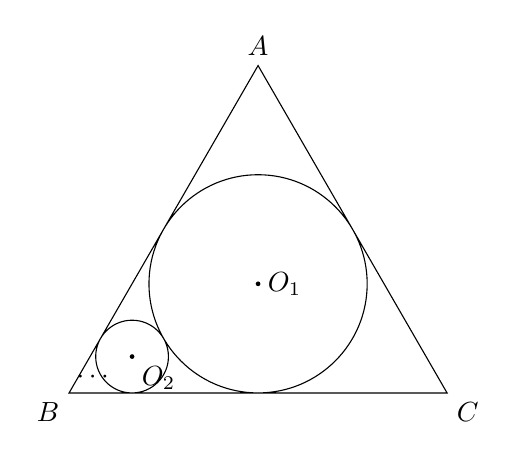
\begin{tikzpicture}[scale=1.2]
\coordinate (B) at (0,0); \coordinate (C) at (4,0); \coordinate (A) at (2,3.464); \coordinate (Oone) at (2,1.1547); \coordinate (Otwo) at (.6667,.3849);
\draw (A)--(B)--(C)--cycle (Oone) circle (1.1547) (Otwo) circle (.3849);
\fill (Oone) circle (.025) (Otwo) circle (.025); \node[right] at (Oone) {$O_1$}; \node[below right] at (Otwo) {$O_2$}; \node[above] at (A) {$A$}; \node[below left] at (B) {$B$}; \node[below right] at (C) {$C$}; \node at (.25,.16) {$\cdots$};
\end{tikzpicture}
